\documentclass{beamer}
\usetheme{default}
%\usetheme{pittsburgh}
\usecolortheme{albatross}

% #####################################################################
% # Saját színek:
\definecolor{todobgszin}{rgb}{0.64,0.78,0.22}
\definecolor{todofrszin}{rgb}{0.00,0.50,0.00}
\definecolor{background}{rgb}{0.00,0.306,0.530}
% #####################################################################

\setbeamercolor{normal text}{fg=white,bg=background}
\setbeamercovered{transparent}
\setbeamertemplate{navigation symbols}{} % Navigációs ikonok off

\usepackage[T1]{fontenc}
\usepackage[utf8]{inputenc}
\usepackage[english,magyar]{babel}

\usepackage{hyperref}
\usepackage{color}
\usepackage{graphics}

\usebackgroundtemplate{

\includegraphics[width=\paperwidth, height=\paperheight]{background.jpg}
}

% Néhány konstans deklarációja:
\newcommand{\vikszerzo}{Nádudvari György}
\newcommand{\vikszerzomail}{ulqp9p@gmail.com}
\newcommand{\vikkonzulens}{Huszerl Gábor}
\newcommand{\vikcim}{Oktatástámogató rendszerek kiszolgáló infrastruktúrájának felügyeleti lehetőségei}
\newcommand{\viktanszek}{Méréstechnika és Információs Rendszerek Tanszék}
\newcommand{\vikdoktipus}{Szakdolgozat}

\newcommand{\setfootline}[1]{\setbeamertemplate{footline}{\setbeamercolor{footline}{fg=white}\begin{beamercolorbox}[sep=1cm,wd=\textwidth,ht=1cm,left]{footline}{#1}\end{beamercolorbox}}}

%###########################################
% Saját eszközök:
%

\newcommand{\todo}[1]{\fcolorbox{todofrszin}{todobgszin}{\emph{TODO: #1}}}
\newcommand{\angolul}[1]{\foreignlanguage{english}{#1}}

\hypersetup{
    bookmarks=true,            % show bookmarks bar?
    unicode=true ,             % non-Latin characters in Acrobat’s bookmarks
    pdftitle={\vikcim},        % title
    pdfauthor={\vikszerzo},    % author
    pdfsubject={\vikdoktipus}, % subject of the document
    pdfcreator={\vikszerzo},   % creator of the document
    pdfnewwindow=true,         % links in new window
    colorlinks=true,           % false: boxed links; true: colored links
    linkcolor=black,           % color of internal links
    citecolor=black,           % color of links to bibliography
    filecolor=black,           % color of file links
    urlcolor=black             % color of external links
}

\title{\vikcim}
\author{\vikszerzo \\ \footnotesize{\texttt{\vikszerzomail}} \\[0.5cm] \normalsize{Konzulens: \vikkonzulens}}
\date{2012. június 14.}

\begin{document}

\section{\vikcim}
\begin{frame}[plain]
\titlepage
\end{frame}

\section{Miről is lesz szó?}
\setfootline{Interstellar Overdrive}
\begin{frame}[t]
\frametitle{Miről is lesz szó?}
\begin{itemize}
    \pause
    \item Tanulásmenedzsment rendszerek
        \begin{itemize}
            \pause
            \item fogalma, feladatai
            \pause
            \item átjárhatóság közöttük és miért fontos ez
        \end{itemize}
    \pause
    \item Tanulásmenedzsment rendszerek IT infrastruktúrája
        \begin{itemize}
            \pause
            \item A három rétegű architektúra a Moodle rendszeren bemutatva
        \end{itemize}
    \pause
    \item Tanulásmenedzsment rendszerek erőforrás igényei
        \begin{itemize}
            \pause
            \item Alapvető igények
            \pause
            \item Modellek
        \end{itemize}
    \pause
    \item Információs technológiai infrastruktúrák
        \begin{itemize}
            \pause
            \item A klasszikus IT infrastruktúra
            \pause
            \item Felhőalapú infrastruktúrák
        \end{itemize}
    \pause
    \item IT infrastruktúrák proaktív menedzsmentje általános és oktatástámogató rendszerek esetén
    \pause
    \item Összefoglalás
\end{itemize}
\end{frame}

\section{Tanulásmenedzsment rendszerek}
\setfootline{Remember a Day}
\begin{frame}[t]
\frametitle{Mik azok a tanulásmenedzsment rendszerek?}
\begin{itemize}
    \pause
    \item Milyen rendszereket nevezünk \angolul{Learning Management Systemnek} (LMS-nek)?
    \pause    
    \item Mik egy LMS feladatai?
    \pause    
    \item Milyen megoldásokat találunk a piacon?
    \pause    
    \item Miért fontos az átjárhatóság?
    \pause    
    \item Mi az a SCORM, és mire jó?
\end{itemize}
\end{frame}

\section{Tanulásmenedzsment rendszerek IT infrastruktúrája}
\setfootline{\todo{@@@@@@@@@@@@@@@@@@@@@@@@@@@@@@@@@@@@@@@@@@@@@}}
\begin{frame}[t]
\frametitle{Tanulásmenedzsment rendszerek IT infrastruktúrája}
\begin{figure}[!ht]
\centering
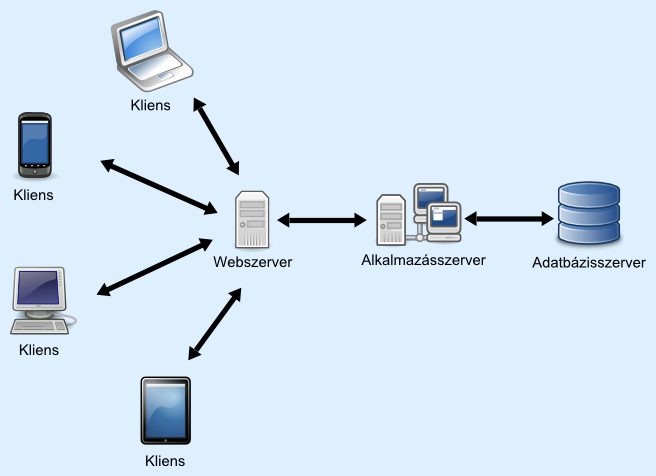
\includegraphics[width=90mm, keepaspectratio]{figures/3tier_simple_001.png}
\end{figure}
\todo{MySQL, Linux, PHP, Moodle logót rátenni a képre!}
\end{frame}

\section{Tanulásmenedzsment rendszerek erőforrás igényei}
\setfootline{\todo{@@@@@@@@@@@@@@@@@@@@@@@@@@@@@@@@@@@@@@@@@@@@@}}
\begin{frame}[t]
\frametitle{Tanulásmenedzsment rendszerek erőforrás igényei}
\begin{itemize}
    \pause
    \item Alapvető igények
    \begin{itemize}
        \pause        
        \item Webszerverek erőforrásigénye
        \pause        
        \item Adatbázisszerverek erőforrásigénye
    \end{itemize}
    \pause
    \item Modellek
    \begin{itemize}
        \pause        
        \item Lehetséges modell alkotások
    \end{itemize}
\end{itemize}
\begin{onlyenv}<7>
\begin{figure}[!ht]
\centering
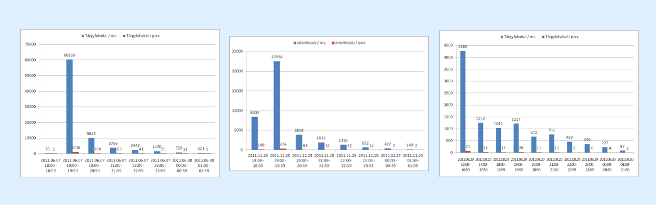
\includegraphics[width=110mm, keepaspectratio]{figures/modellek.png}
\end{figure}
\end{onlyenv}
\end{frame}

\section{Információs technológiai infrastruktúrák}
\setfootline{\todo{@@@@@@@@@@@@@@@@@@@@@@@@@@@@@@@@@@@@@@@@@@@@@}}
\begin{frame}[t]
\frametitle{Információs technológiai infrastruktúrák}
\begin{itemize}
    \pause
    \item A klasszikus IT infrastruktúra
    \begin{itemize}
        \pause
        \item Adatbázis réteg
        \begin{itemize}
            \pause            
            \item terheléselosztás (load balancing)
            \pause
            \item replikálás
            \pause
            \item feladatátadás hiba esetén (failover) 
        \end{itemize}
        \pause
        \item Alkalmazás réteg
        \pause
        \item Webkiszolgáló réteg
    \end{itemize}
    \pause
    \item Virtualizáció
    \pause
    \item Felhőalapú infrastruktúrák
\end{itemize}
\end{frame}

\section{IT infrastruktúrák proaktív menedzsmentje általános és oktatástámogató rendszerek esetén}
\setfootline{\todo{@@@@@@@@@@@@@@@@@@@@@@@@@@@@@@@@@@@@@@@@@@@@@}}
\begin{frame}[t]
\frametitle{IT infrastruktúrák proaktív menedzsmentje általános és oktatástámogató rendszerek esetén}
\end{frame}

\section{Összefoglalás}
\setfootline{\todo{@@@@@@@@@@@@@@@@@@@@@@@@@@@@@@@@@@@@@@@@@@@@@}}
\begin{frame}[t]
\frametitle{Összefoglalás}
\end{frame}

\section{A bíráló kérdése}
\setfootline{\todo{@@@@@@@@@@@@@@@@@@@@@@@@@@@@@@@@@@@@@@@@@@@@@}}
\begin{frame}[t]
\frametitle{A bíráló kérdése}
\textbf{Kérdés}:
\begin{itemize}
\item Hogyan specifikálná (vagy hogyan véleményezné) azokat az intézményi igényeket (szerzői jogok, biztonsági szempontok, stb.) amikor már nem javasolt az LMS futtatása a felhőalapú infrastruktúrán?
\end{itemize} 
\textbf{Válasz}:
\begin{itemize}
\item Léteznek kezdeményezések, megoldások a probléma megoldására
\end{itemize}
\todo{Ezen gondolkodni, Gáborral egyeztetni!}
\end{frame}

\section{Kérdések}
\setfootline{\todo{@@@@@@@@@@@@@@@@@@@@@@@@@@@@@@@@@@@@@@@@@@@@@}}
\begin{frame}[t]
\frametitle{Kérdések}
\end{frame}

\section{Vége}
\setfootline{\todo{@@@@@@@@@@@@@@@@@@@@@@@@@@@@@@@@@@@@@@@@@@@@@}}
\begin{frame}[c]
\frametitle{}
\begin{center}
\huge{\textbf{Köszönöm a figyelmet!}}
\end{center}
\end{frame}

\end{document}
